\documentclass{article}
\usepackage{bm}
\usepackage{amsmath}
\usepackage{graphicx}
\usepackage{mdwlist}
\usepackage[colorlinks=true]{hyperref}
\usepackage{geometry}
\geometry{margin=1in}
\geometry{headheight=2in}
\geometry{top=2in}
\usepackage{palatino}
%\renewcommand{\rmdefault}{palatino}
\usepackage{fancyhdr}
%\pagestyle{fancy}
\rhead{}
\lhead{}
\chead{%
  {\vbox{%
      \vspace{2mm}
      \large
      Introduction to Deep Learning M2177.0043 \hfill
\\
      Seoul National University
      \\[4mm]
      Homework \#(\textbf{1})\\
      \textbf{Hwapyeong Song}
    }
  }
}

\graphicspath{{.}}

\usepackage{paralist}

\usepackage{todonotes}
\setlength{\marginparwidth}{2.15cm}

\usepackage{tikz}
\usetikzlibrary{positioning,shapes,backgrounds}

\begin{document}
\pagestyle{fancy}

\section*{INSTRUCTIONS}

\begin{itemize*}
\item Anything
  that is received after the deadline will be considered to be late and we do not receive late homeworks. We do however ignore your lowest homework grade. 
\item Answers to every theory questions need to be submitted
  electronically on ETL. Only PDF generated from LaTex is accepted.
\item Make sure you prepare the answers to each question
  separately. This helps us dispatch the problems to different graders.
\item Collaboration on solving the homework is allowed. Discussions
  are encouraged but you should think about the problems on your own. 
\item If you do collaborate with someone or use a book or website, you
  are expected to write up your solution independently.  That is,
  close the book and all of your notes before starting to write up
  your solution.
\end{itemize*}

%!TEX root = hw1.tex

%% Q1
\section{Q1. Learning \LaTeX{}}
\subsection{2 by 2 table}
  \begin{tabular}{|c|c|}
    \hline
    Hwapyeong & Song \\
    \hline
    Department of English Language and Literature & 2014-15703 \\
    \hline
  \end{tabular}


\subsection{Profile photo}
  \begin{center}
    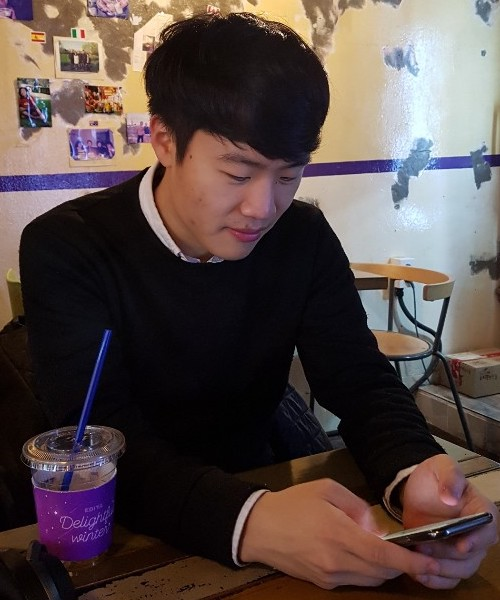
\includegraphics[scale=0.25]{profile_picture}
  \end{center}

  %% Q2
\section{Q2. Inverse transform sampling}
\subsection{Probability integral transform}
By definition of continous uniform distribution, if the random variable $Y = F_X(X)$ is uniformly distributed in $[0, 1]$, $F_Y(y) = y$ for all $y \in [0, 1]$ and vice versa.
As $F_X(x)$ is defined to be equal to $Pr[X \leq x]$, $F_Y(y) = Pr[Y \leq y]$. Random variable Y is defined as $F_X(X)$, thus
$F_Y(y) = Pr[Y \leq y] = Pr[F_X(X) \leq y]$. There may be many values such that $F_X(X) \leq y]$. If we denote such values as $F_X^{-1}([0, 1])$, then $Pr[F_X(X) \leq y]$
can be written as $Pr[X \in F_X^{-1}([0, y])]$, thus $F_Y(y) = Pr[X \in F_X^{-1}([0, y])]$.

As $F_X$ is continous, there exists a supremum in $F_X^{-1}([0, y])$, and as this is a closed set, this is also a maximum. Let this maximum value be denoted as $k$, such that $k = max(F_X^{-1}([0, y]))$.
Then, $F_Y(y) = Pr[X \in F_X^{-1}([0, y])] = Pr[X \leq k] = F_X(k) = y$ as we defined $k$ to be a maximum element such that $F_X^{-1}([0, y])$.

\subsection{Inverse transform sampling}
Let a random variable $V = F_X^{-1}(U)$. By definition of continuous uniform distribution, $F_V(x) = Pr[V \leq x]$. If $F$ is applied to the both sides in $V = F_X^{-1}(U)$, then we get $U = F_X(V)$.
Therefore $Pr[V \leq x] = Pr[U \leq F_X(x)]$. As $U$ is given as a uniform distribution in $[0, 1]$, $Pr[U \leq F_X(x)] = F_X(x)$. Thus $F_V(x) = F_{F_X^{-1}(U)}(x) = Pr[F_X^{-1}(U) \leq x] = F_X(x)$,
implying that $F_X(x)$ is a CDF of $F_X^{-1}(U)$. 

\subsection{Sampling from exponential distribution}
$f(x; \frac{1}{\beta}) = \frac{1}{\beta} \exp(-\frac{x}{\beta}),$

%% Q3
\section{Q3}

%% Q4
\section{Q4}


\end{document}
